\chapter{Evaluation} \label{chap:Evaluation}
In this chapter, various case studies are introduced which demonstrate the use of an extension. They have been chosen in order to illustrate the important features of CRI and therefore the contributions of this thesis. We have collected examples written using RxJS and BaconJS libraries from the internet. We have evaluated the extension against 8 RxJS and 2 BaconJS applications and we present the results in this section. We focus on features provided by our extension and evaluate that feature with the applications. In the last section, we summarize and conclude the evaluation.

\section{Operators}
Operators play important role in both libraries. Developers can use operators to transform, filter and many other operations. To demonstrate how CRI helps developers to understand reactive applications, we have taken RxJS operators example. This section also illustrates the evolution of dependency graph for the given example.

\subsection{RxJS - Operators}
In our example, we have selected \textit{map}, \textit{filter} and \textit{last} operators from RxJS library. One can find use case of other operators in RxJS official documentation\footnote{\url{http://reactivex.io/documentation/operators.html}}. Dependency graph generated by CRI after executing the program is shown in figure \ref{fig:rxjs-operators-dg}. In the following example~\ref{lst:rxjs-operators}, \textit{source} is an observable with values 1,2,3,4,5. In line 3, \textit{map} operator is applied, which maps each values from an observable and adds 10 to each value and new MapObservable is created. At line 5, \textit{filter} operator filters the even values out of MapObservable. The \textit{last} operator at line 7 receives values 12 and 14 after applying filter operator and emits value 14 which the last value in observable. At line 9, subscriber \textit{subscribe} is subscribing to \textit{example} observable. Thus, \textit{subscribe} will receive value 14 and is printed to console in line 10.

\begin{lstlisting}[language=JavaScript, caption=RxJS - Operators example, label={lst:rxjs-operators}]
var source = Rx.Observable.from([1, 2, 3, 4, 5]);
// apply map, filter and last operator
var example = source.map(function (val) {
	return val + 10;
}).filter(function (num) {
	return num % 2 === 0;
}).last();
//output: "Last to pass test: 14"
var subscribe = example.subscribe(function (val) {
	return console.log("Last value: " + val);
});
\end{lstlisting}

\begin{figure}[!h]
	\centering
	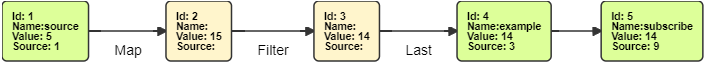
\includegraphics[scale=0.7,trim=0 0 0 0]{images/RxJS-operators/final.png}
	\caption{Dependency graph - RxJS Operators example}
	\label{fig:rxjs-operators-dg}
\end{figure}

As we said earlier, CRI helps developer understand flow of reactive applications. For example~\ref{lst:rxjs-operators}, evolution of dependency graph can be depicted as shown in figure \ref{fig:rxjs-operators-dg-evolution}. Developer can use the provider slider to navigate to and forth to visualize evolution of graph.

\begin{figure}[!h]
	\centering
	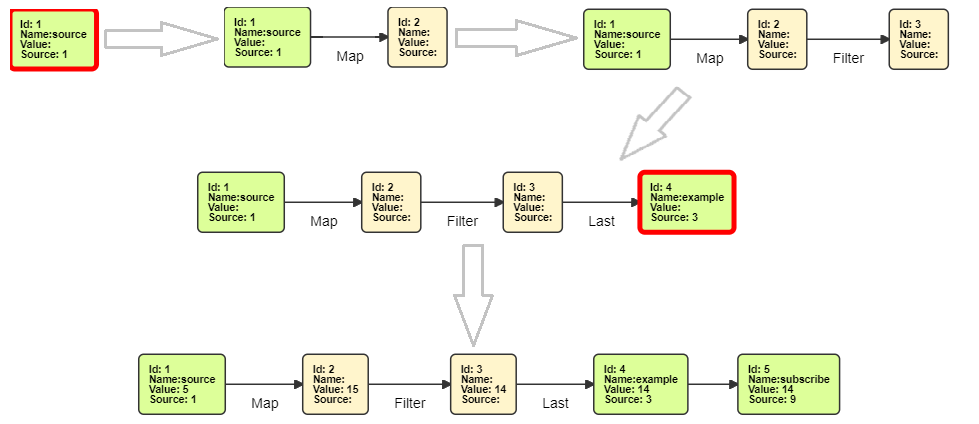
\includegraphics[scale=0.7,trim=0 0 0 0]{images/RxJS-operators/steps-all.png}
	\caption{Dependency graph evolution - RxJS Operators example}
	\label{fig:rxjs-operators-dg-evolution}
\end{figure}

\section{RxJS - Simple Data-binding example}
Listing \ref{lst:rxjs-data-binding} shows relevant javascript code for this example. In this example, user enters data in two HTML input fields, firstname and lastname. Output of the application is combination of both names. The UI of an application looks as shown in figure~\ref{fig:sd-ui} and Dependency graph is shown in figure~\ref{fig:sd-dg}. 

\begin{lstlisting}[language=JavaScript, caption=RxJS - Databinding example, label={lst:rxjs-data-binding}]
// Create simple bindings for first and last name
var firstName1 = new Rx.BehaviorSubject('');
var lastName1 = new Rx.BehaviorSubject('');

// Create first and last name composite
var fullName1 = firstName1.combineLatest(lastName1, function (first, last) {
	return first + ' ' + last;
});

// Subscribe to them all
var fn1 = document.querySelector('#firstName1');
firstName1.subscribe(function (text) { fn1.value = text });

var ln1 = document.querySelector('#lastName1');
lastName1.subscribe(function (text) { ln1.value = text });

var full1 = document.querySelector('#fullName1');
fullName1.subscribe(function (text) { full1.value = text });

// Create two way bindings for both first name and last name
Rx.Observable.fromEvent(fn1, 'keyup')
.subscribe(function (e) { firstName1.next(e.target.value); })

Rx.Observable.fromEvent(ln1, 'keyup')
.subscribe(function (e) { lastName1.next(e.target.value); })
\end{lstlisting}


\begin{figure}[!h]
	\centering
	\subfloat[UI]{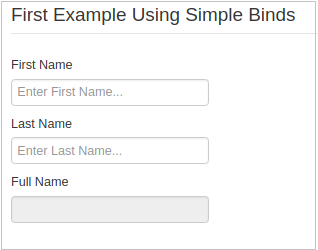
\includegraphics[width=0.4\textwidth]{images/simple-data-binding/simple_db_UI.png}\label{fig:sd-ui}}
	\hfill
	\subfloat[Dependency graph]{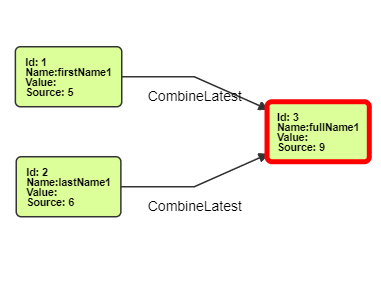
\includegraphics[width=0.4\textwidth]{images/simple-data-binding/sd-dg.png}\label{fig:sd-dg}}
	\caption{Simple Data-binding example - RxJS}
\end{figure}

// To be continued